\begin{figure}[t]
\centering
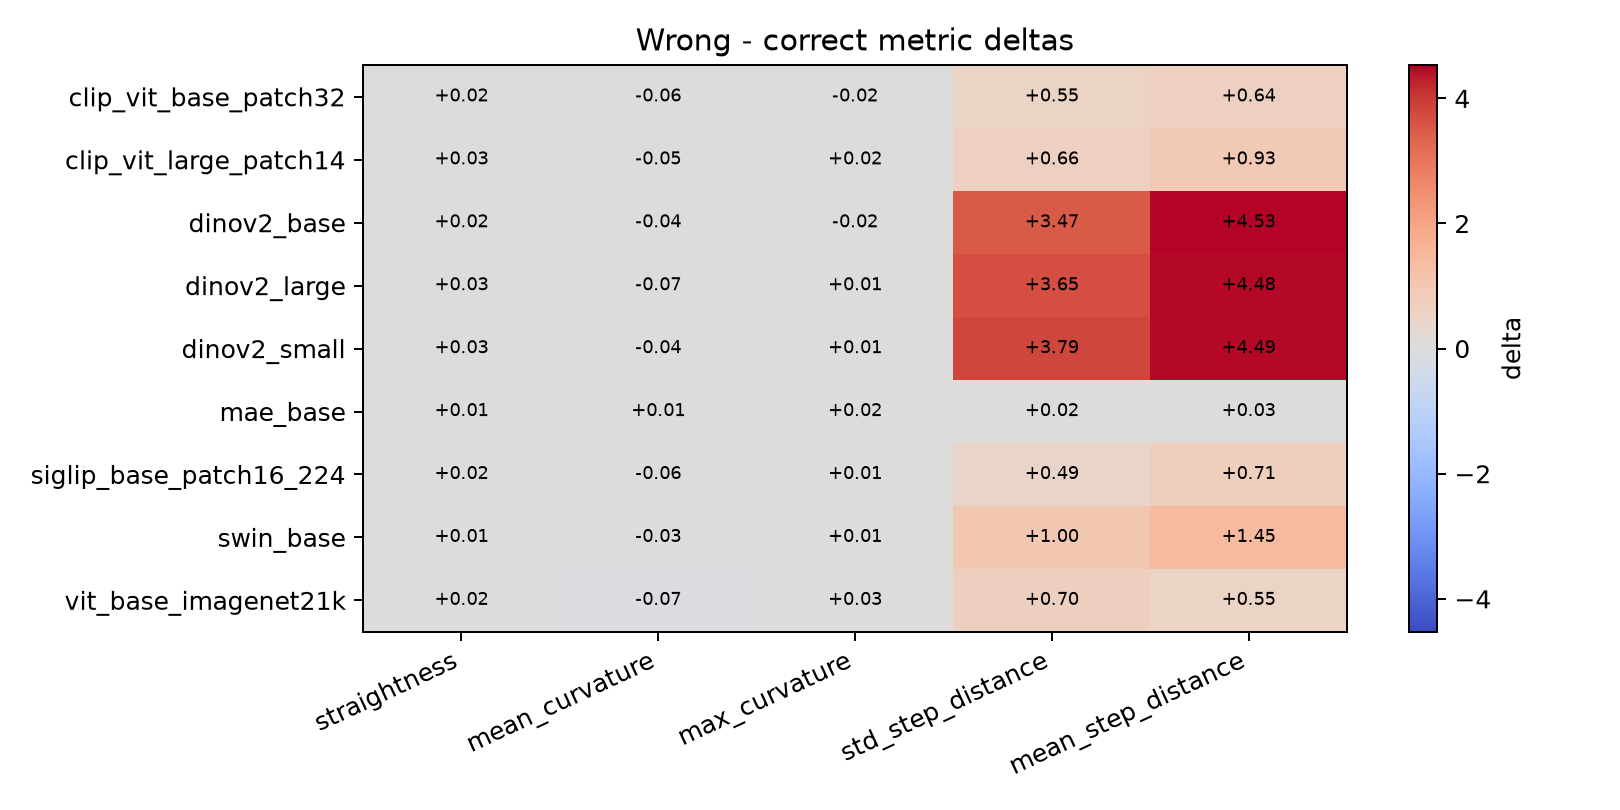
\includegraphics[width=\linewidth]{generated/simulated_pendulum/figures/delta_heatmap.png}
\caption{Wrong-minus-correct metric deltas across encoders on the simulated pendulum benchmark. The step-distance metrics show the most consistent positive changes for wrong-physics videos, while straightness and curvature are less stable.}
\label{fig:sim-delta-heatmap}
\end{figure}

\begin{figure}[t]
\centering
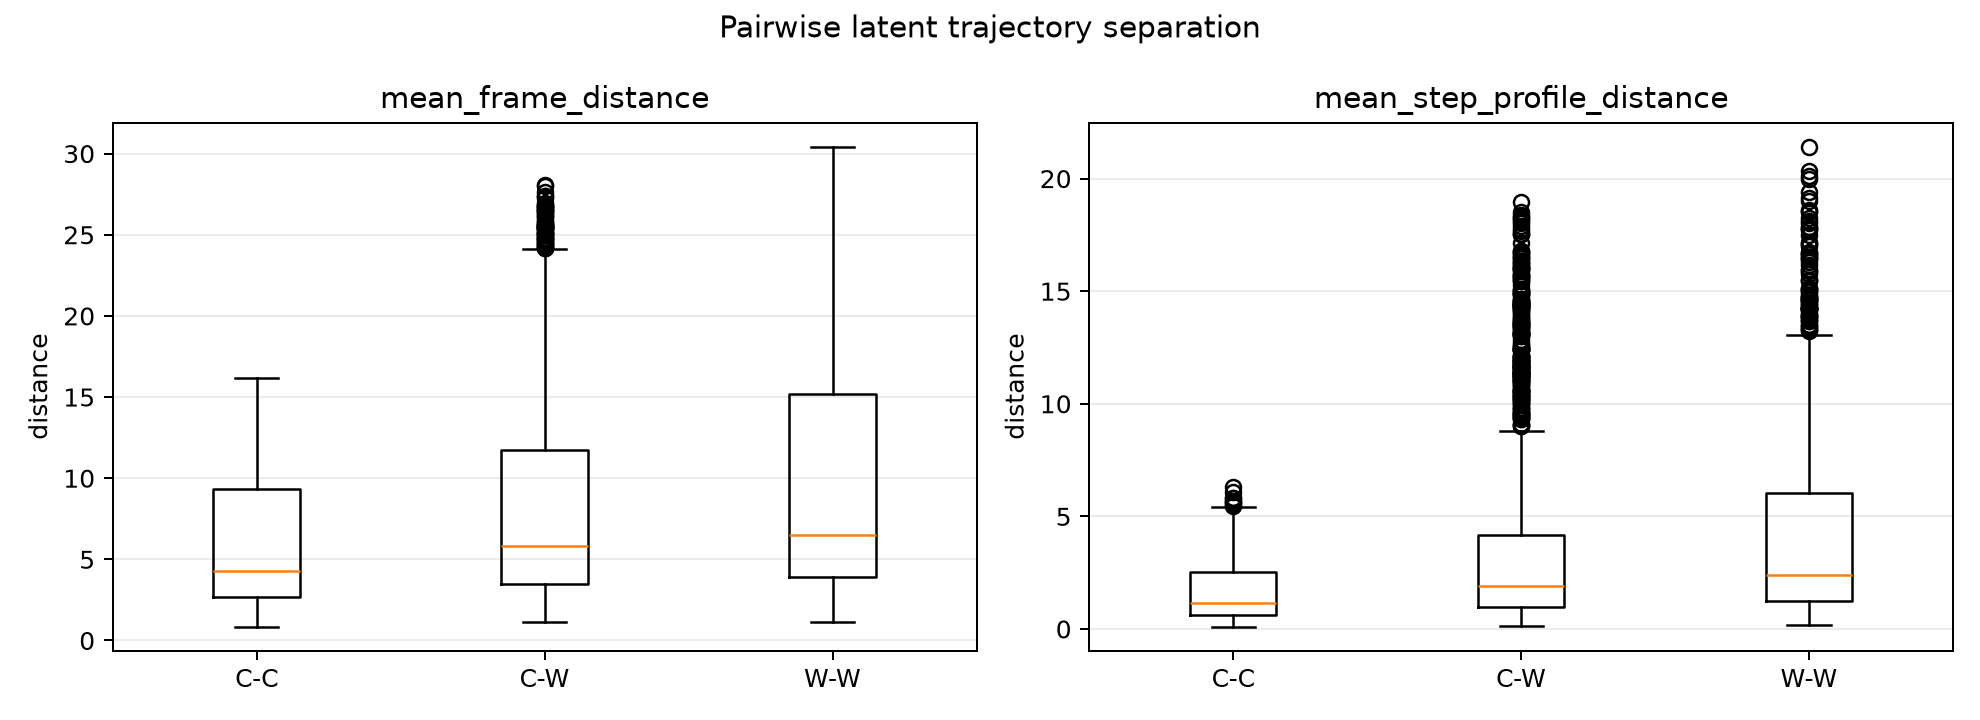
\includegraphics[width=\linewidth]{generated/simulated_pendulum/figures/pairwise_separation.png}
\caption{Pairwise latent trajectory separation. Correct-wrong pairs are compared against correct-correct pairs to test whether physical violations exceed normal variation between simulated correct videos.}
\label{fig:sim-pairwise-separation}
\end{figure}

\begin{figure}[t]
\centering
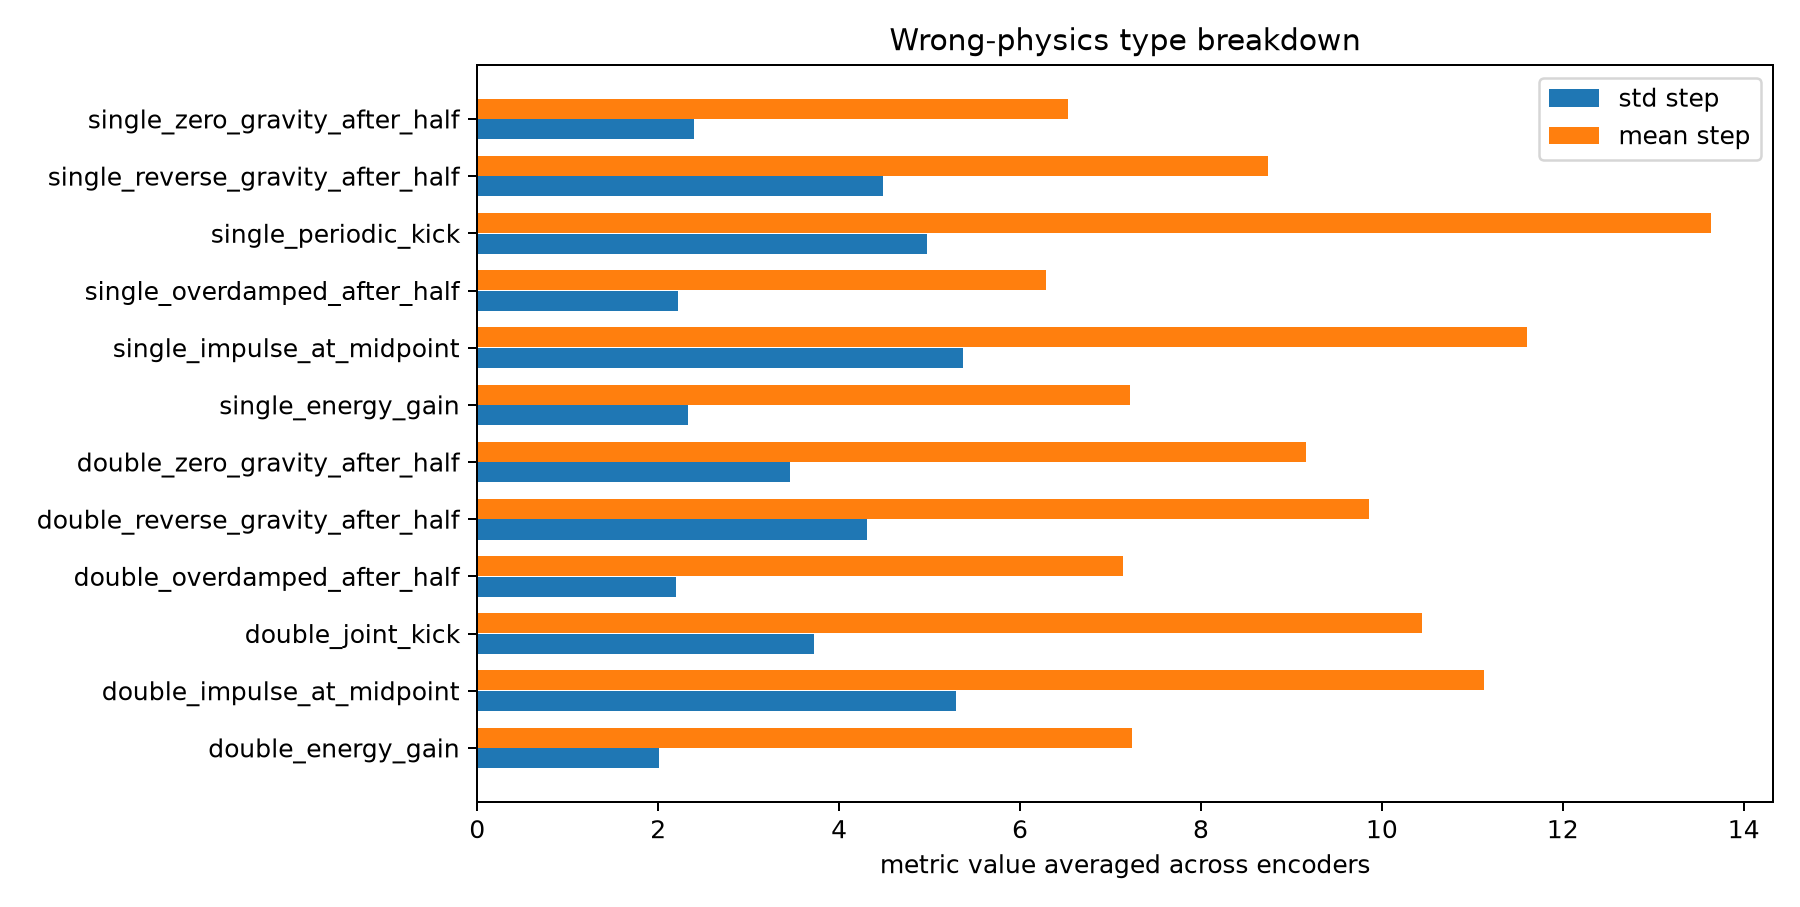
\includegraphics[width=\linewidth]{generated/simulated_pendulum/figures/wrong_type_step_distance.png}
\caption{Wrong-physics type breakdown. Abrupt interventions such as velocity kicks and gravity changes produce stronger latent movement than smoother perturbations.}
\label{fig:sim-wrong-type-breakdown}
\end{figure}

\begin{figure}[t]
\centering
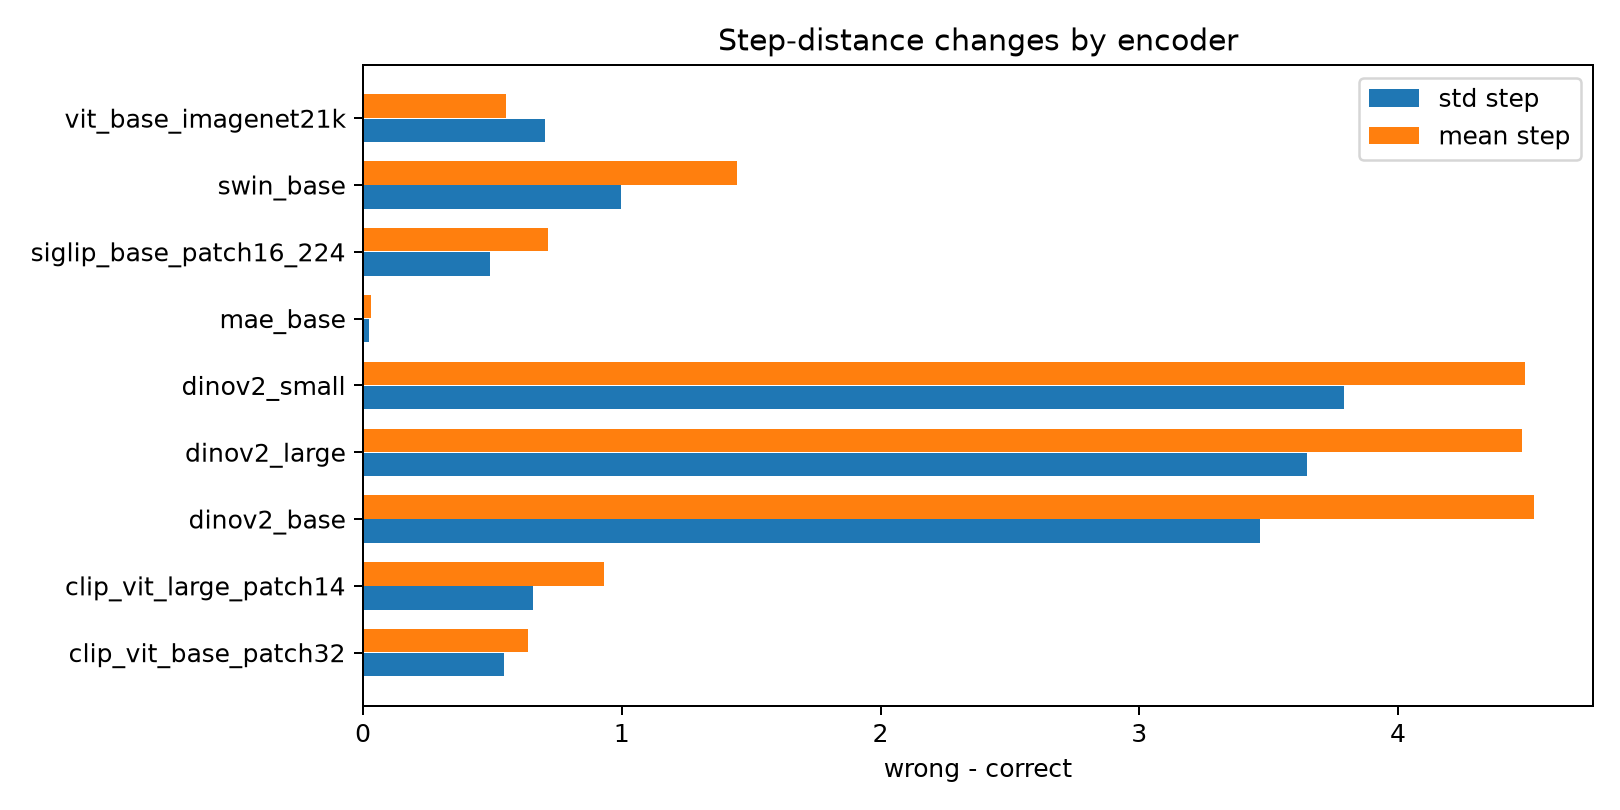
\includegraphics[width=\linewidth]{generated/simulated_pendulum/figures/encoder_step_deltas.png}
\caption{Encoder-wise changes in mean and standard deviation of frame-to-frame latent step distances. DINOv2 encoders show the largest absolute step-distance changes, while MAE does not separate correct and wrong physics in this setting.}
\label{fig:sim-encoder-step-deltas}
\end{figure}

\begin{figure}[t]
\centering
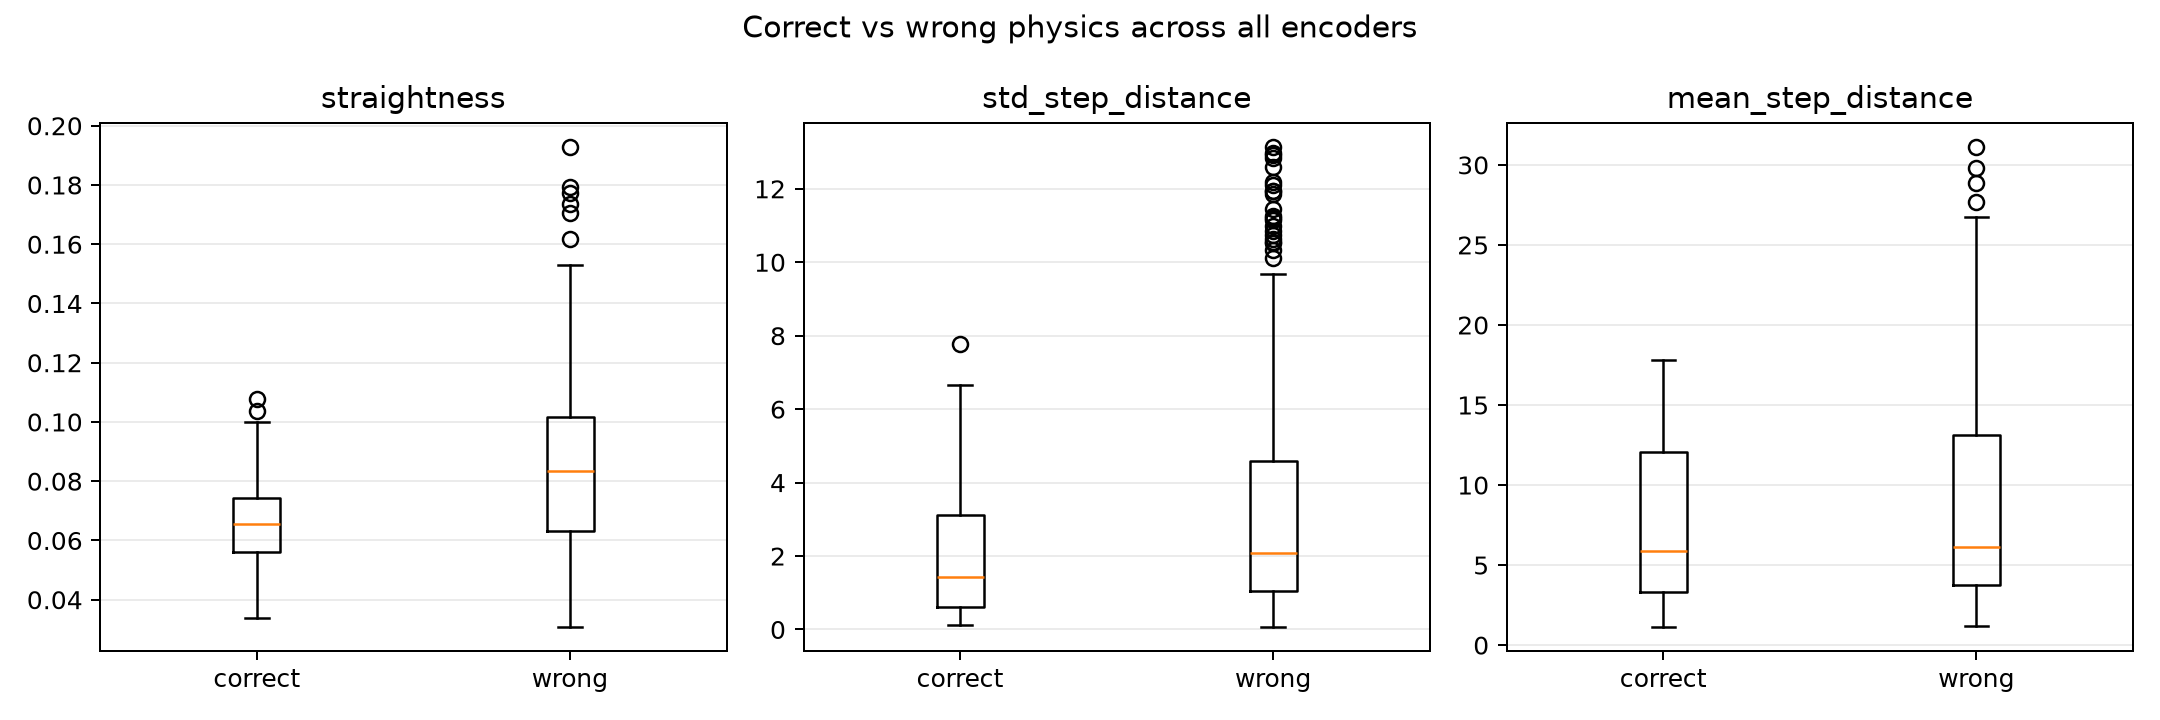
\includegraphics[width=\linewidth]{generated/simulated_pendulum/figures/metric_boxplots.png}
\caption{Correct versus wrong metric distributions pooled across encoders. Straightness overlaps strongly between the two classes, whereas wrong-physics videos produce a heavier upper tail for step-distance variability.}
\label{fig:sim-metric-boxplots}
\end{figure}

\begin{figure}[t]
\centering
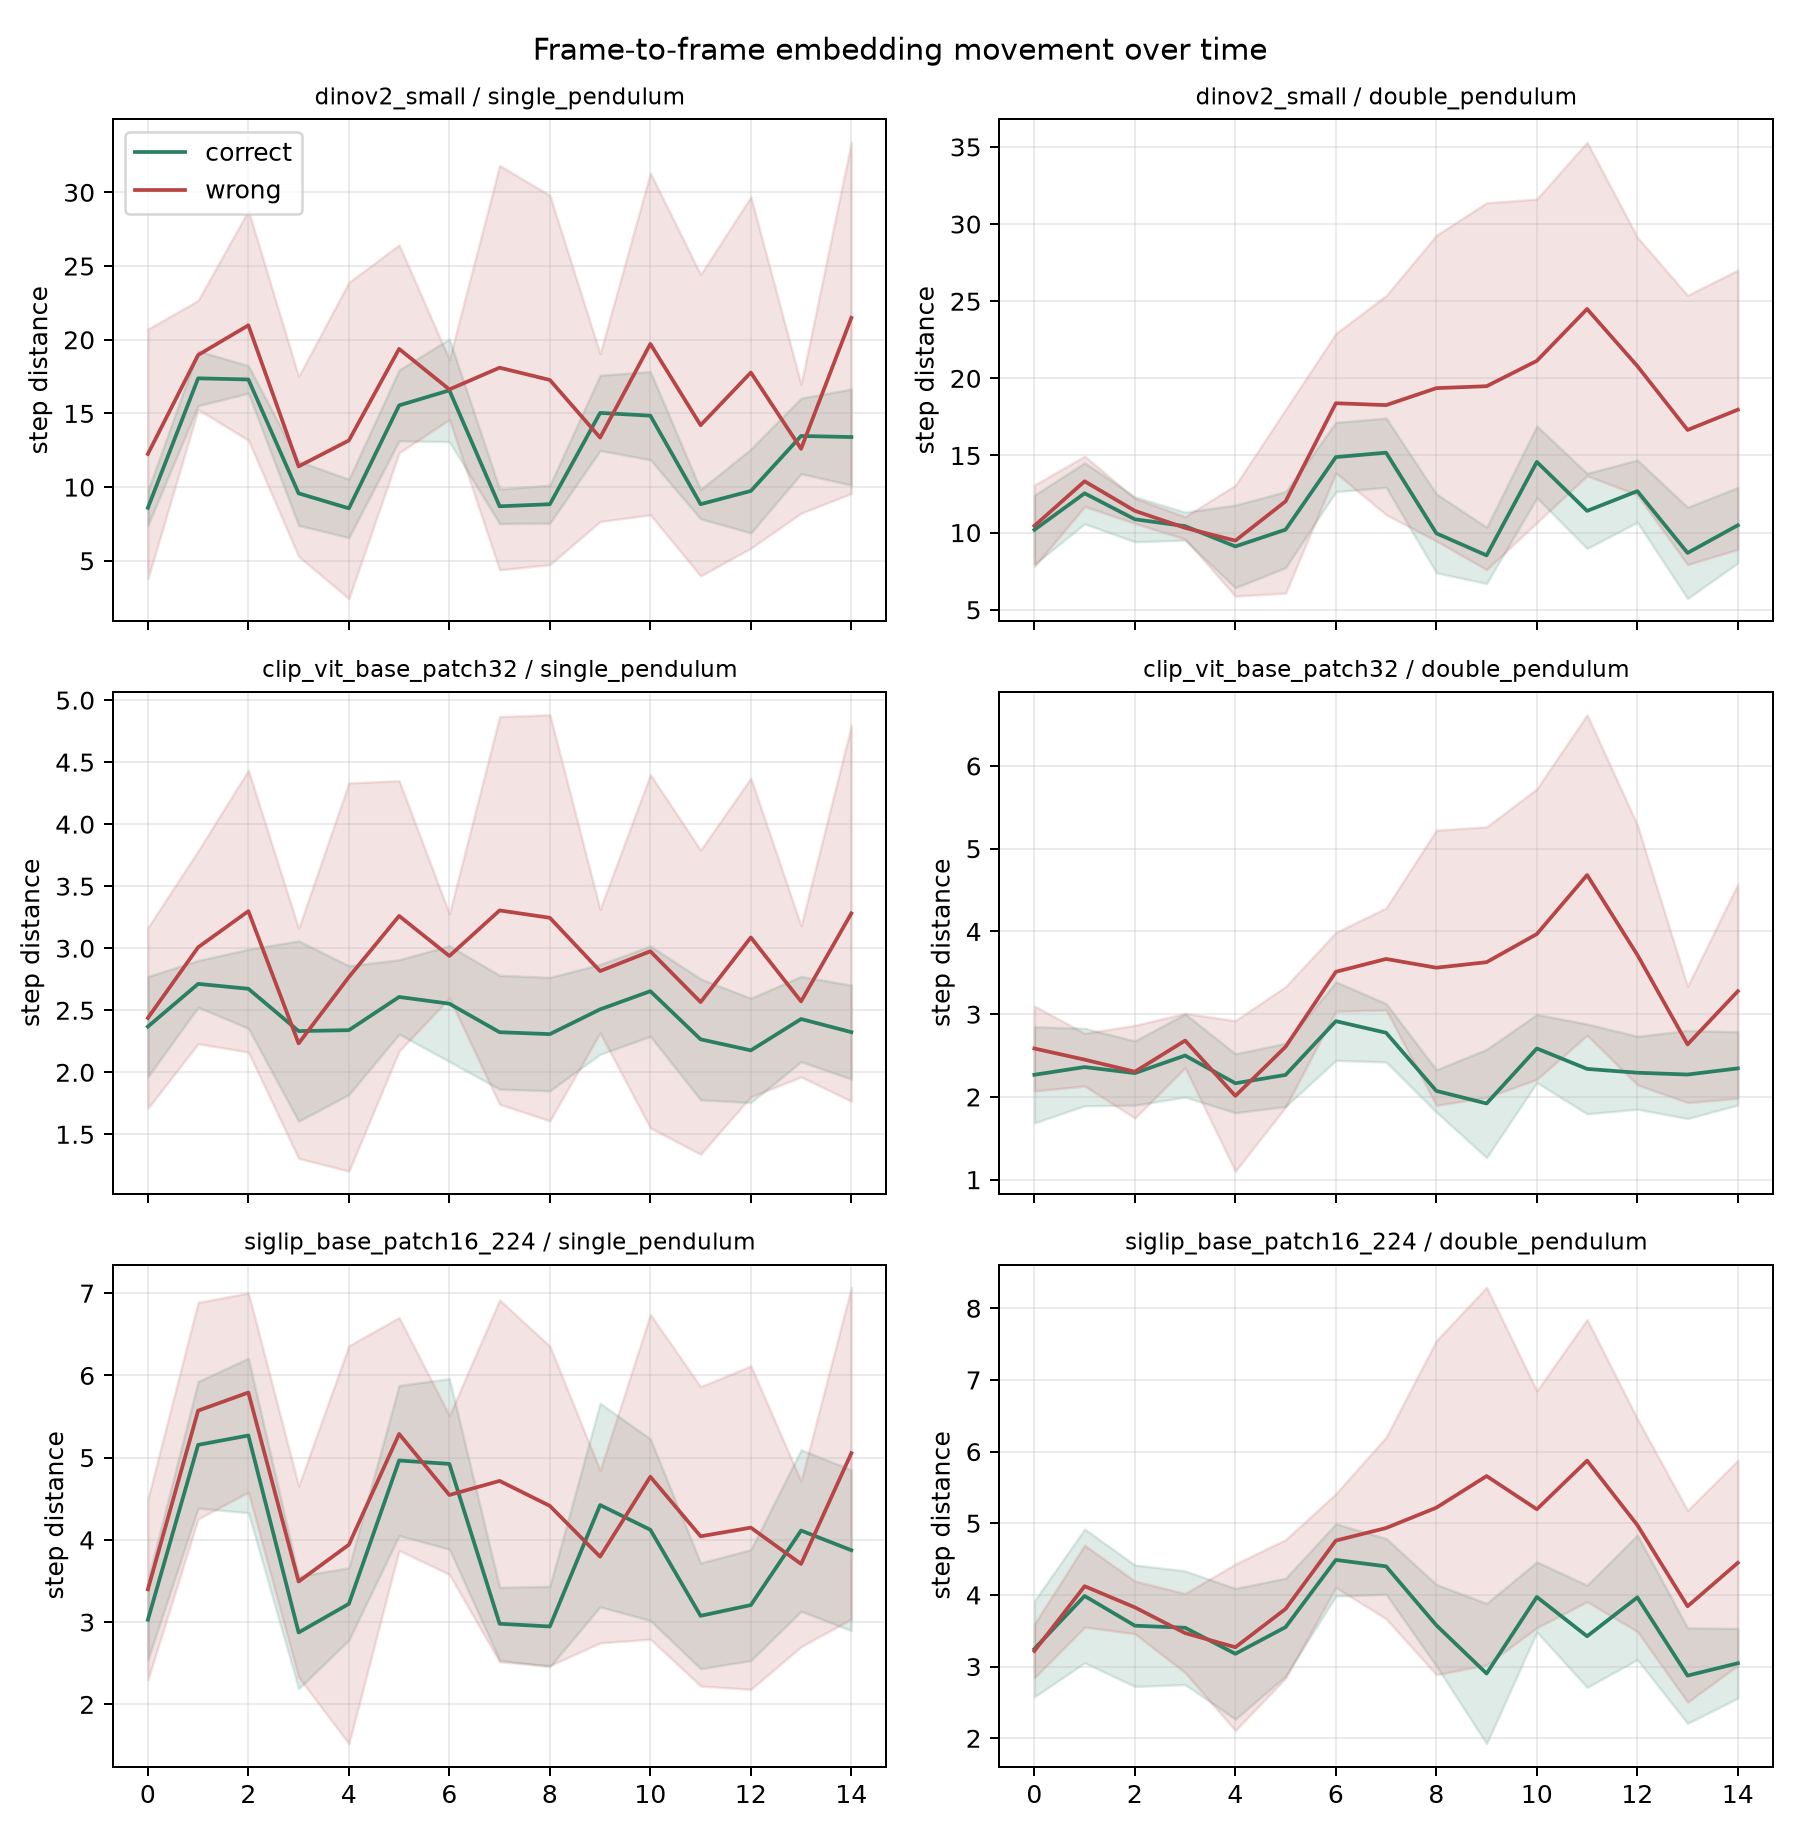
\includegraphics[width=\linewidth]{generated/simulated_pendulum/figures/step_distance_timeseries.png}
\caption{Temporal profile of frame-to-frame latent movement for representative encoders. Wrong-physics videos tend to have larger movements and occasional spikes, especially for DINOv2-small and CLIP-B/32.}
\label{fig:sim-step-timeseries}
\end{figure}

\begin{figure}[t]
\centering
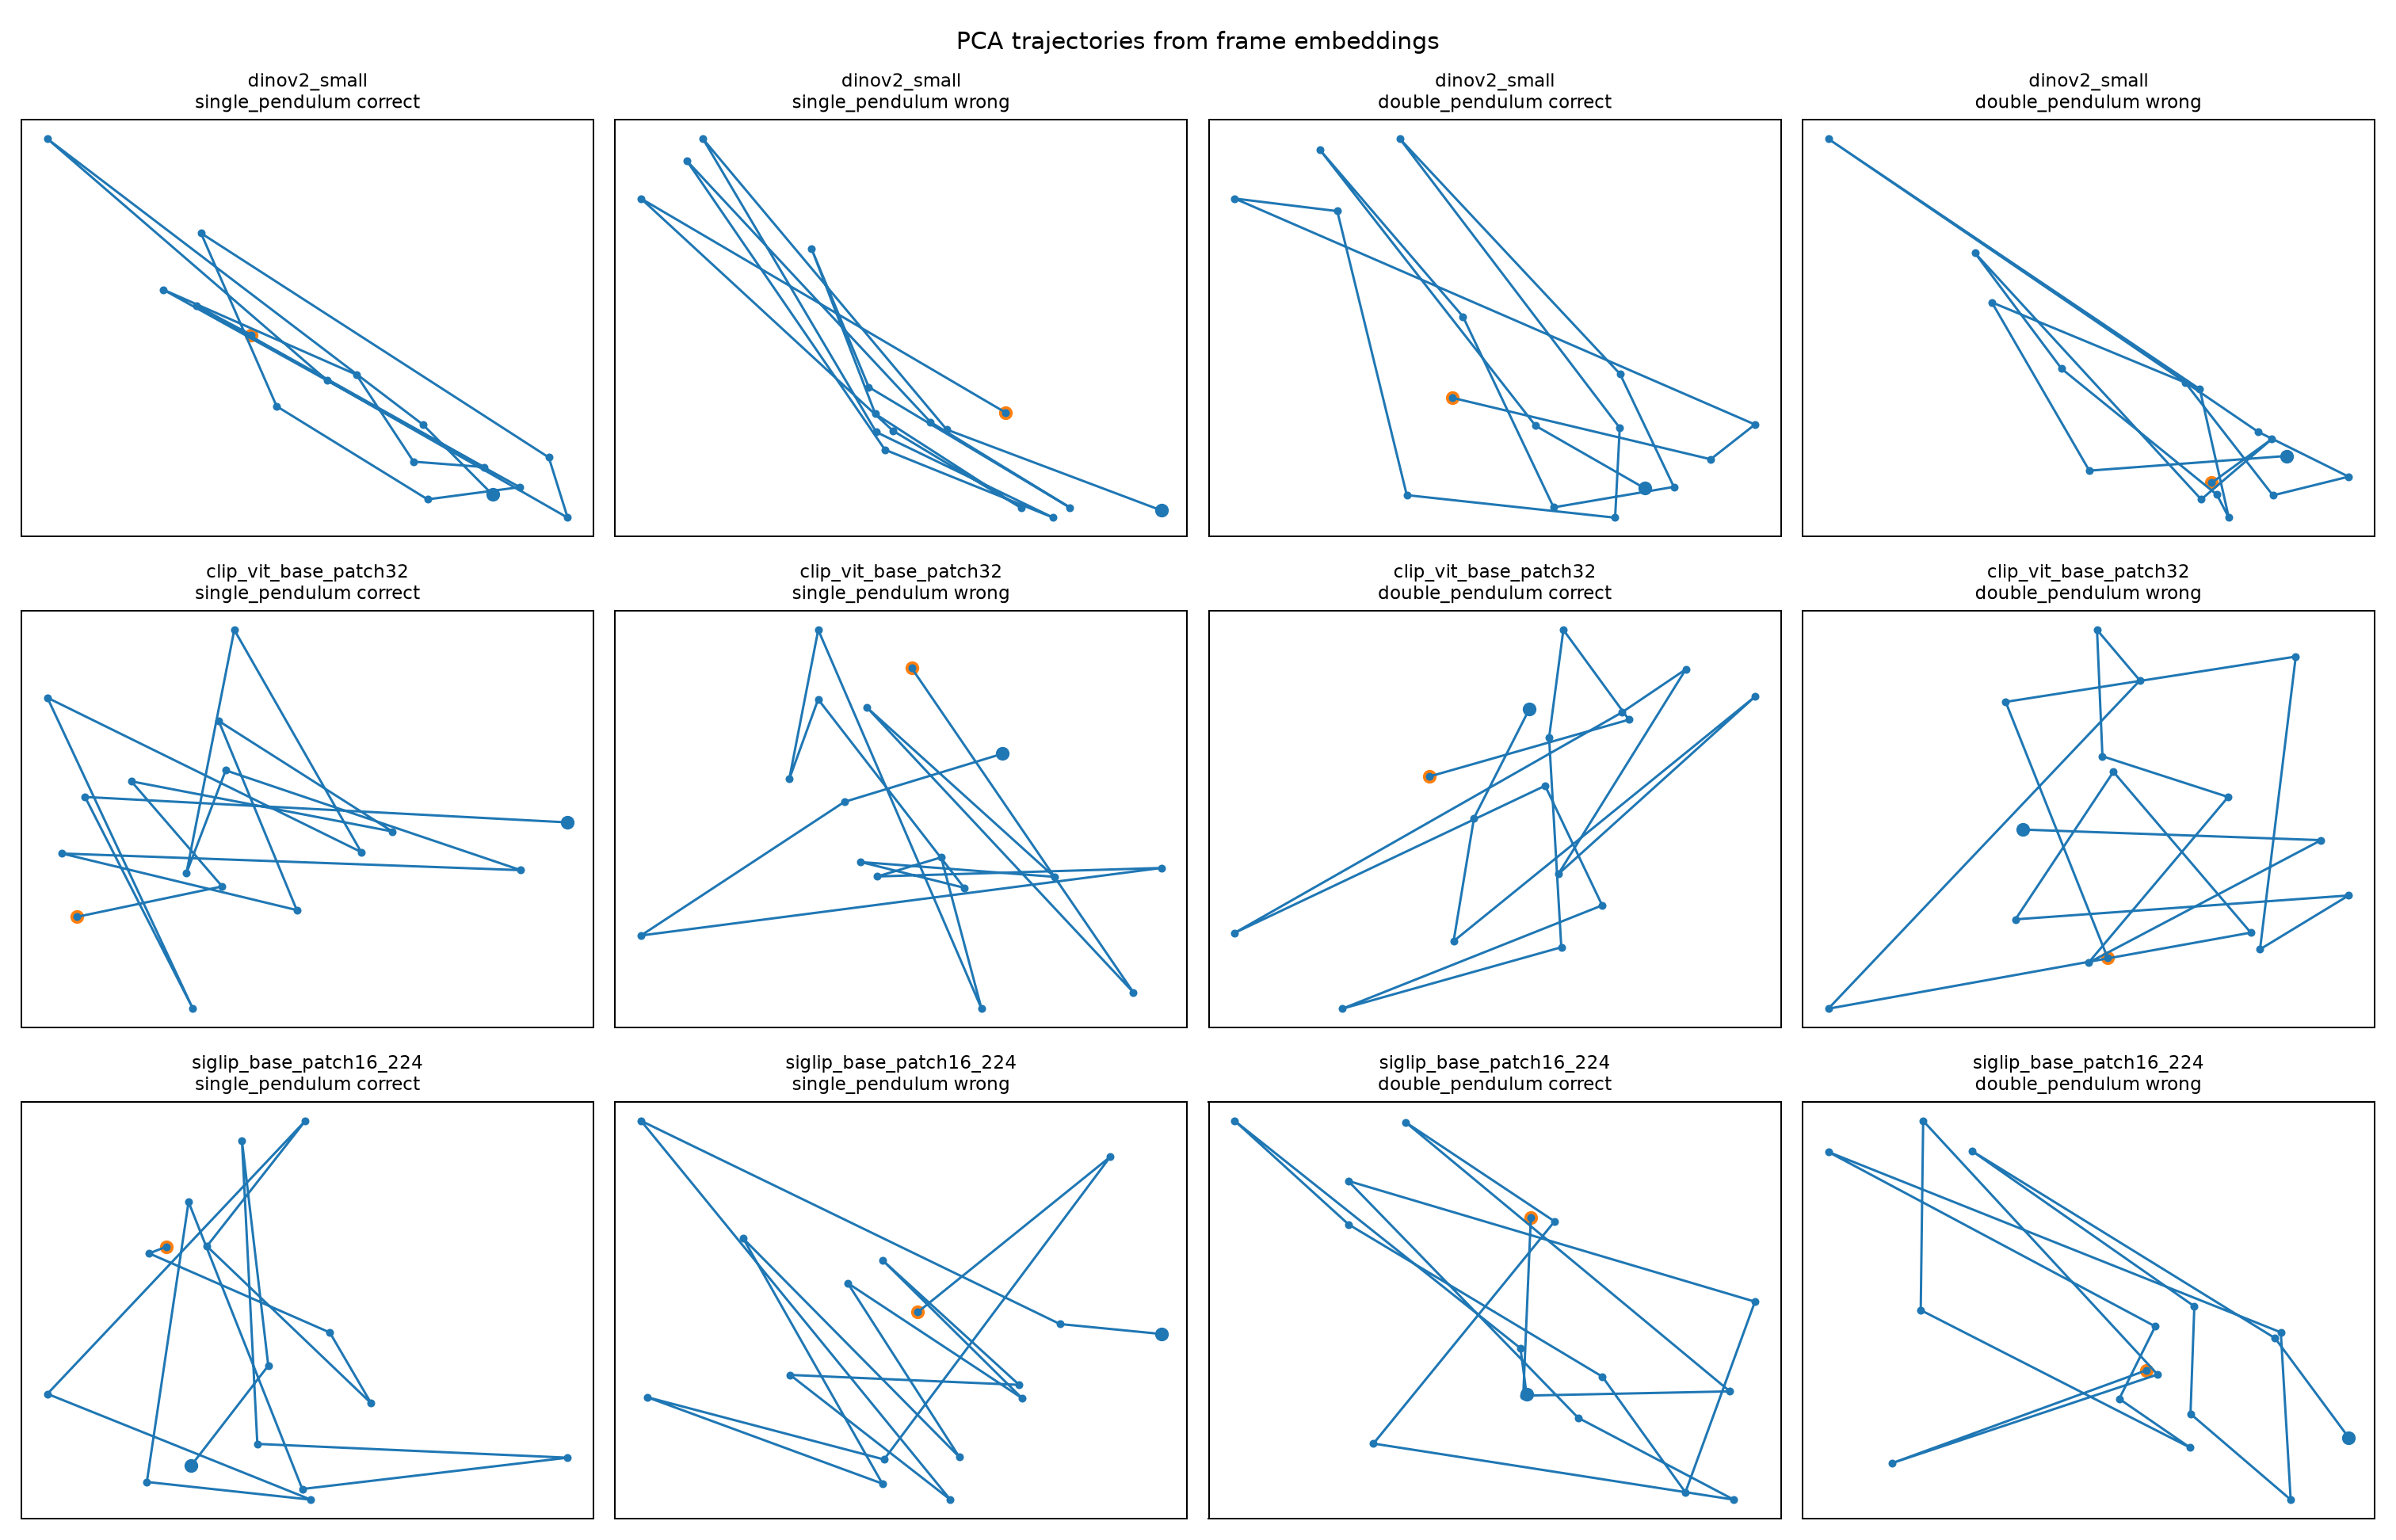
\includegraphics[width=\linewidth]{generated/simulated_pendulum/figures/pca_trajectories.png}
\caption{Qualitative PCA visualisation of selected latent trajectories. Each point is a sampled frame embedding. This figure is intended as an illustration of trajectory behaviour rather than the primary quantitative evidence.}
\label{fig:sim-pca-trajectories}
\end{figure}

\begin{figure}[t]
\centering
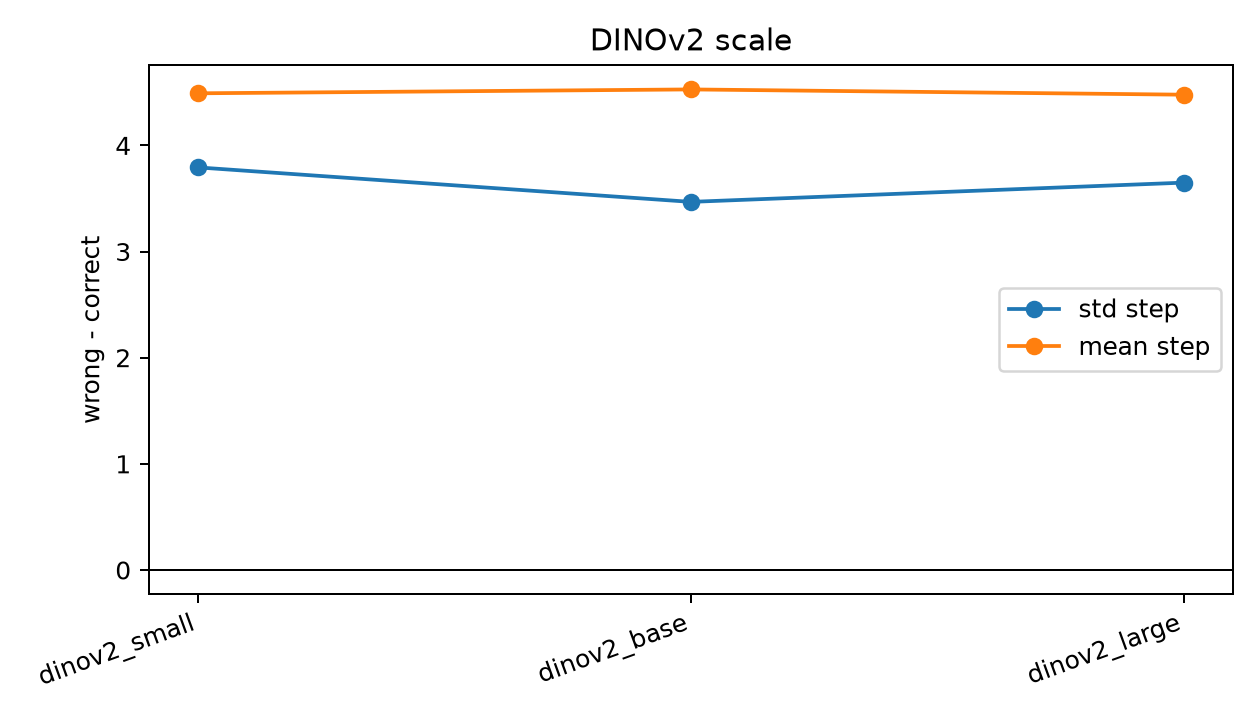
\includegraphics[width=0.48\linewidth]{generated/simulated_pendulum/figures/dinov2_scale.png}
\hfill
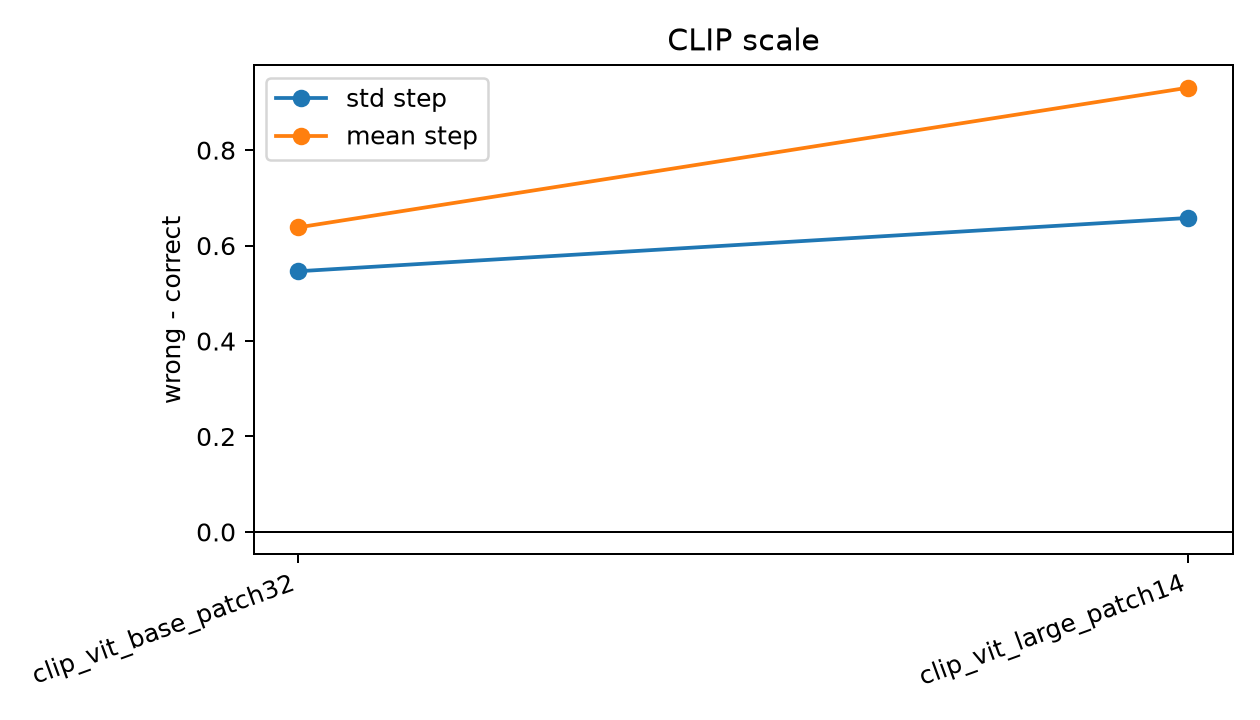
\includegraphics[width=0.48\linewidth]{generated/simulated_pendulum/figures/clip_scale.png}
\caption{Model-scale comparisons for DINOv2 and CLIP. DINOv2 models consistently show positive step-distance deltas, but the effect is not monotonic with scale. CLIP-B/32 is more separable than CLIP-L/14 in this benchmark.}
\label{fig:sim-scale-comparison}
\end{figure}
